\documentclass[pdf,bluish,slideColor,colorBG]{prosper}
\hypersetup{pdfpagemode=FullScreen}
\usepackage{graphicx}
\usepackage{color}
%\usepackage{amsfonts}
\def\baselinestretch{0.7}
\parindent 0.3in
\hyphenpenalty=10000
\tolerance=10000
\pagestyle{empty}

\definecolor{purple}{rgb}{1.0,0.0,1.0}
\definecolor{golden}{rgb}{1.0,0.8,0.3}
\definecolor{gold}{rgb}{0.9,0.6,0.3}
\definecolor{red}{rgb}{1.0,0.0,0}

\title{Systematics and molecular evolution:}
\subtitle{some history of numerical methods}
\author{Joe Felsenstein}
\institution{Department of Genome Sciences and Department of Biology\\
University of Washington, Seattle}

\begin{document}

\def\Prob{{\rm Prob\;}}
\def\prob{{\rm \;Prob\;}}


\maketitle

\begin{slide}[Replace]{Irrelevant?}

In the 1960's molecular biologists commonly considered all population
biology as an irrelevancy at best: mere ``stamp collecting"

\bigskip

\centerline{\fbox{\parbox[t]{3in}{In science there is only physics,\\
 all else is stamp collecting\\
\hspace*{0in} {~~} \hfill {\it Ernest Rutherford}}}}

\bigskip

By contrast, while molecular biologists ignored evolutionary biology until
the 1990s,
population biologists had been using molecular methods since the
late 1960's, but to a degree limited by their limited funding.

\end{slide}

\begin{slide}[Replace]{The problem}

Population biologists have been working on numerical methods for
inferring phylogenies (evolutionary trees) since the 1960's.  Their
importance has
only recently been recognized by molecular biologists.

The inference of, and use of phylogenies is a central problem in
computational molecular biology, though in bioinformatics textbooks
they usually are covered in only a small part of the book (usually
just a few pages).

\end{slide}

\begin{slide}[Replace]{Why evolution?}

\begin{center}
\framebox{\parbox[t]{2.8in}{Nothing in biology makes sense\\
except in the light of evolution.\\
\hspace*{0in} \hfill {\it Theodosius Dobzhansky, 1973}}}
\end{center}
\bigskip

\bigskip

Perhaps that is an overstatement (what about physics and chemistry?), but evolution is how
the data came to be, and taking evolution into account is the only efficient
way of analyzing it.

\end{slide}

\begin{slide}[Replace]{Ernst Mayr and George Gaylord Simpson}

\centerline{\includegraphics[width=1.0in]{mayr1953.ps} \hspace{0.4in}
\includegraphics[width=1.25in]{simpson.ps}}
\bigskip

\centerline{\hspace*{0in}\hspace{0.2in}Ernst Mayr (1905-2005) \hspace{0.2in} George Gaylord Simpson (1902-1984)}
\medskip

\begin{itemize}
\item Major figures in the completion of the ``modern synthesis'' or ``Neodarwinian
synthesis'' in the 1940s.
\item Leaders of the ``evolutionary systematics''
approach to taxonomic classification, dominant until the 1970s.
\end{itemize}

\end{slide}

\begin{slide}[Replace]{Evolutionary-systematic classification}
\bigskip

\centerline{\includegraphics[height=2.3in]{mayrsimpson.idraw}}
\bigskip


A pattern of grades with very unequal rates of overall evolution is implicit
in the use of paraphyletic groups in Mayr and Simpson's practice.

\end{slide}

\begin{slide}[Replace]{A horse tree drawn by Simpson}

\centerline{\includegraphics[width=1.8in]{horses.ps}}
\medskip

\centerline{(tree fading away -- it is getting obese and nonspecific.)}

\end{slide}

\begin{slide}[Replace]{Willi Hennig (1913-1976) }

\centerline{\includegraphics[width=1.5in]{Hennig3.ps}}
\medskip

The major advocate and developer of ``phylogenetic systematics'' which
advocates that all groups be monophyletic.  Outlined a simple method
for inferring phylogenies that can be used when characters do not conflict.

\end{slide}

\begin{slide}[Replace]{Positions on classification as of about 1960}

\begin{itemize}
\item \textcolor{purple}{Evolutionary systematics.} ~ George Gaylord Simpson and Ernst Mayr
led a movement that allowed non-monophyletic (paraphyletic) groups such
as reptiles, on the assumption that groups could be separated by real
differences of rates of evolution (sometimes ``grades'' rather than ``clades''). 
But did molecular data show similar differences of rates of evolution as
morphology?
\item \textcolor{purple}{Phylogenetic systematics.} ~ Willi Hennig advocated purely monophyletic
classification.
\item \textcolor{purple}{Phenetics.} ~ Sokal and Sneath advocated making a classification without
reference to evolution, using numerical clustering methods
\end{itemize}

\end{slide}

\begin{slide}[Replace]{Technological change post World War II}
\bigskip

\begin{itemize}
\item Former physicists found molecular biology (first protein sequence, 1951)
\item Former codebreakers and atomic bomb builders build the early
computers (first stored-program digital computer, 1949)
\item Most U.S. universities got their first computer about 1957.
\item First sequences of same gene in multiple species in late 1950s.
\end{itemize}



\end{slide}

\begin{slide}[Replace]{Molecular evolution gets off the ground}

Zuckerkandl and Pauling in 1962 discussed using trees to infer ancestral
sequences, and named this ``chemical paleogenetics".  They were about
30 years ahead of their time.

\begin{center}
\begin{tabular}{c c}
{
\includegraphics[height=1.3in]{Zuckerkandl1986.ps}} &
{\includegraphics[height=1.3in]{pauling.ps}} \\
\parbox[t]{1.5in}{Emile Zuckerkandl\\in 1986} &
\parbox[t]{2.0in}{Linus in 1962, {\it from\\ Nobel Peace Prize web page}} \\
\end{tabular}
\end{center}
\medskip

(But then it isn't fair to anyone to compare them unfavorably to Linus Pauling).

\end{slide}


\begin{slide}[Replace]{Peter Sneath in 1962 and Robert Sokal in 1964}

\begin{center}
\begin{tabular}{r l}
\includegraphics[height=1.9in]{sneath2.ps} &
\includegraphics[height=1.9in]{rrs5a.ps}
\end{tabular}
\end{center}
\medskip

Developers in the late 1950s and early 1960s of numerical clustering methods and chief originators and
advocates of the ``phenetic'' approach to classification, which clusters
organisms by similarity without reference to evolutionary history.

\end{slide}

\begin{slide}[Replace]{The first numerical phylogeny: Sokal and Michener 1957}

\begin{center}
\includegraphics[width=3.0in]{sokaltree.ps}
\end{center}

A tree of bees, which Michener intended as an inference of the phylogeny.

\end{slide}

\begin{slide}[Replace]{Cavalli-Sforza and Edwards, 1963; Edwards, 1970}

\begin{center}
\begin{tabular}{r l}
\includegraphics[height=2in]{cavedwards3.ps} &
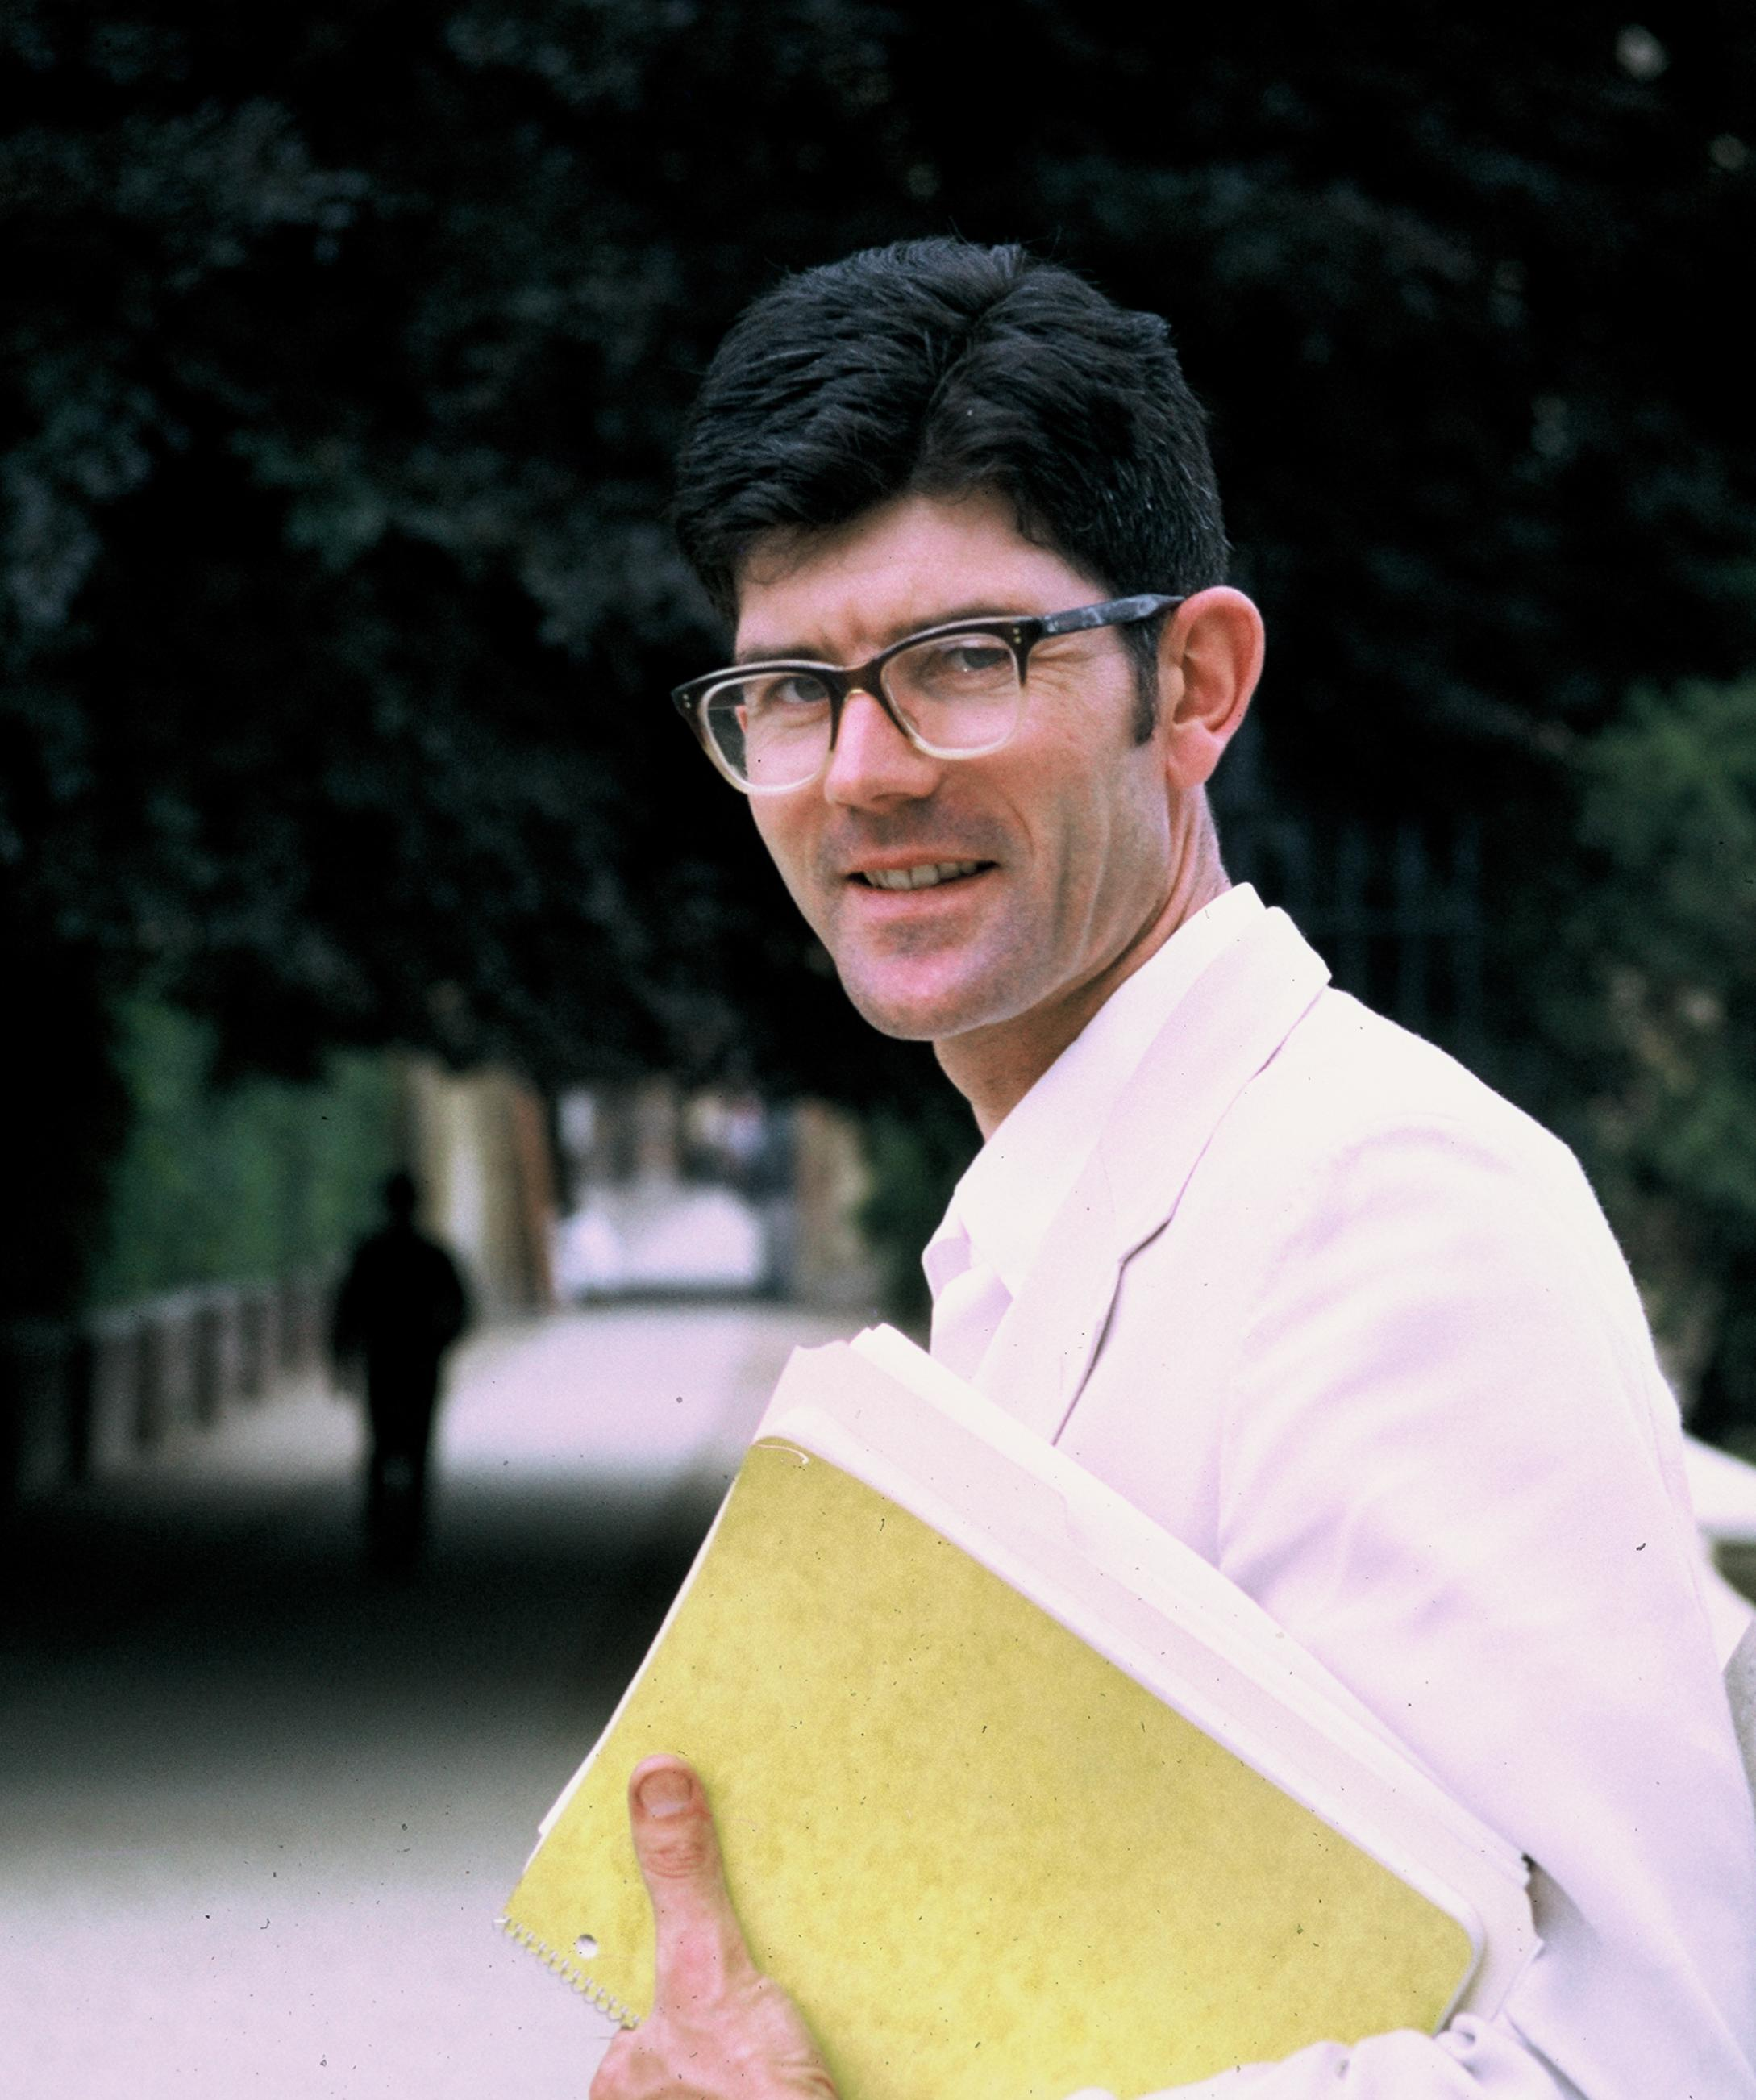
\includegraphics[height=2in]{edwards6.ps}
\end{tabular}
\end{center}
\medskip

Introduced (in 1963-1964) the parsimony and likelihood methods for inferring phylogenies,
and were co-inventors (with Fitch and Margoliash) of the distance matrix
methods.  These are the three major methods for reconstructing phylogenies.

\end{slide}

\begin{slide}[Replace]{The first phylogeny by parsimony}

\begin{center}
\includegraphics[width=2.8in]{edwardstree3.ps}
\end{center}

Gene frequencies of human populations, the tree of minimum length in gene
frequency space, inferred by Edwards and Cavalli-Sforza.

\end{slide}

\begin{slide}[Replace]{Camin in the 1970s, one of the Caminalcules}

\begin{center}
\begin{tabular}{c c}
\includegraphics[height=1.9in]{camin3.ps} &
\includegraphics[height=1.9in]{caminalcule.ps}
\end{tabular}
\end{center}
\medskip

Camin noticed (in 1965) that students who did the best job recovering the true
``phylogeny'' of the Caminalcules made the reconstruction which required the
fewest changes of state.

\end{slide}

\begin{slide}[Replace]{J. S. Farris and Arnold Kluge in the 1980s}

\begin{center}
\includegraphics[height=1.7in]{Farris3b.ps} \includegraphics[height=1.7in]{kluge.ps}
\end{center}
\medskip

Further developments of parsimony methods, starting in 1969, advocacy of them and of Hennig's
approach to classification during the 1970s and on.  Central in the rise (in 1980) of the Willi Hennig Society.

\end{slide}

\begin{slide}[Replace]{Margaret Dayhoff (1925-1983)}
\centerline{\includegraphics[height=1.5in]{dayhoff2.ps}}
\medskip

\centerline{Margaret Dayhoff in about 1966. {\it Courtesy of Ed Dayhoff.}}
\medskip

{\ptsize{8}
\begin{itemize}
\item A major pioneer of molecular databases (starting in 1965)
\item (With Richard Eck) made the first numerical phylogenies using molecular data
\item Presented trees organized by gene families in the {\it Atlas of Protein
Sequences} (later the PIR database) in 1966.
\item Compiled the first empirical substitution rate matrices for amino acids,
intended to form the basis of a probabilistic model of protein evolution.
\end{itemize}
}

\end{slide}

\begin{slide}[Replace]{Walter Fitch: distance methods and DNA parsimony}

\begin{center}
\begin{tabular}{c c}
& \includegraphics[height=2.0in]{Fitch3a.ps}\\
\end{tabular}
\end{center}

Walter Fitch (1929-2011) :

{\ptsize{8}
\begin{itemize}
\item The first major distance matrix method (1967)
\item Developed algorithm (1971) that counts changes of state in DNA parsimony.
\item Introduced the terms and concepts of orthology and paralogy.
\item Co-founded the journal MBE and the SMBE.
\end{itemize}
}

\end{slide}

\begin{slide}[Replace]{Fitch and Margoliash's 1967 distance tree}

\begin{center}
\includegraphics[width=1.7in]{fitchtree.ps}\\
\includegraphics[width=1.7in]{fitchcaption.ps}\\
\end{center}

\end{slide}

\begin{slide}[Replace]{Thomas Jukes and Charles Cantor (middle) in the 1990s}

\begin{center}
\includegraphics[height=1.8in]{jukes.ps} \includegraphics[height=1.8in]{cantor.ps}
\end{center}
\medskip

In 1969 Jukes and Cantor introduced the first stochastic process model
of DNA change, as one paragraph buried in the midst of a giant review of
protein sequence evolution.
\medskip

Cantor later made important technical discoveries in genomics.  Jukes was
a nutritional biochemist who was the primary person responsible for insisting
that pregnant women get folic acid in their diet.

\end{slide}

\begin{slide}[Replace]{Jerzy Neyman}

\centerline{\includegraphics[height=2in]{neyman.ps}}
\medskip

A major figure in mathematical statistics (confidence intervals, Neyman-Pearson
testing theorems), Neyman was enticed in 1971
into doing the first likelihood analysis of molecular sequence data for
protein sequences with a 3-species tree and a Jukes-Cantor-like symmetrical
model of change among 20 amino acids.

\end{slide}

\overlays{8}{
\begin{slide}[Replace]{Further development of statistical methods}
\bigskip

\begin{itemstep}
\item ``Pruning'' algorithm for efficient calculation of likelihoods on trees
(me, 1973, but not yet applied to molecules)
\item Proof of inconsistency of parsimony (me, 1978; James Cavender too, 1978)
\item Programs distributed (WAGNER78, JS Farris 1978; PHYLIP, me, 1980; PAUP,
Swofford, 1983)
\item Pruning algorithm used to make ML work for DNA (me, 1981)
\item Bootstrap and other sampling methods assess confidence of clades (me,
1985; Penny and Hendy, 1985)
\item Neighbor-Joining method (Nei and Saitou, 1987)
\item Codon models (Goldman and Yang, 1994; Muse and Gaut, 1994)
\item AIC model comparison (Adachi and Hasegawa, 1996; Posada and Crandall, 1998)
\item Bayesian MCMC phylogenies (Yang/Rannala/Mau/Newton/Larget/Li/Pearl/Doss, 1997-2000)
\end{itemstep}
\end{slide}
}

\begin{slide}[Replace]{Sources of work on molecular phylogenies}
\bigskip

\centerline{\includegraphics[width=3.8in]{molevol.idraw}}

A noticeable tendency is for much of the influence to come from
outside systematics, and for biochemists (as opposed to ``molecular
biologists'') to be an important
influence on work in molecular evolution.

\end{slide}

\overlays{6}{
\begin{slide}[Replace]{Conflict over phylogeny methods, 1970s to 1980s}

\begin{itemstep}
\item Hennig's 1950 book {\it Grundz\"uge einer Theorie der phylogenetischen
Systematik} is translated as {\it Phylogenetic Systematics} in 1966.
\item Advocacy of his views is taken up by a number of systematists (Brundin,
Nelson, Platnick) in the 1970s.
\item Some numerical systematists, chiefly J. S. Farris, ally with them.
\item They adopt an evangelical and messianic style and attack entrenched evolutionary
systematists, calling themselves ``phylogenetic systematists''.
\item Tensions between phylogenetic systematists and others within the 
Numerical Taxonomy Conference lead to major conflicts
at its 1979 meeting at Harvard University.  Not a fun meeting.
\item They found a separate organization, the Willi Hennig Society, in 1980
(today their house journal is {\it Cladistics})
\end{itemstep}

\end{slide}
}
\overlays{5}{
\begin{slide}[Replace]{More conflict over phylogeny methods, 1980s to today}

\begin{itemstep}
\item Many other numerically-oriented people found themselves
outside this group.
\item Molecular evolutionists mostly avoided these conflicts and
have remained pragmatic and eclectic.
\item After about 1990, the SSB
and the SMB became the
gathering points for all the folks who were outside of the Will Hennig
Society, Many were
phylogenetic systematists, but they wanted normal
scientific communication.
\item In the 1990s use of likelihood and
Bayesian methods (and distance methods interpreted statistically)
gradually became
recognized as ``statistical phylogenetics'', an alternative to the Hennig Society's parsimony-only approach to
reconstructing phylogenies.
\item The Hennig Society spurns compromise and has centers of strength
among morphological systematists (e.g. AMNH in New York; Cornell University).
\end{itemstep}

\end{slide}
}

% \begin{slide}[Replace]{Did Hennig invent parsimony?}
% 
% \begin{quote}
% Unfortunately, AIV is not sufficiently detailed to allow us to select a
% unique criterion for choosing a most preferable tree.  We know that trees on
% which the monophyletic groups share many steps are preferable to trees on
% which this is not so.  But AIV deals only with single monophyletic groups 
% and does not tell us how to evaluate a tree consisting of several
% monophyletic groups.  One widely used criterion -- parsimony -- could be used
% to select trees.  This would be in accord with AIV, since on a most
% parsimonious tree OTUs [tips] that share many states (this is {\it not} the
% same as the OTUs' being {\it described} by many of the same {\it states})
% are generally placed together.  We might argue that the parsimony criterion
% selects a tree most in accord with AIV by ``averaging" in some sense the
% preferability of all the monophyletic groups of the tree.  Other criteria,
% however, may also agree with AIV.
% \end{quote}
% 
% \begin{flushright}
% Farris, Eckardt and Kluge, 1970
% \end{flushright}
% 
% \end{slide}
% 
\begin{slide}[Replace]{Positions on classification nowadays}

\begin{itemize}
\item \textcolor{purple}{Phylogenetic systematics.} ~ Willi Hennig advocated purely monophyletic
classification.  Now the (strongly) dominant approach.
\item \textcolor{purple}{Evolutionary systematics.} ~ Has almost faded away.  Its adherents were
reluctant to make it algorithmic.
\item \textcolor{purple}{Phenetics.} ~ Although Sokal and Sneath strongly influenced the field of
numerical clustering, their approach to biological classification has few
adherents.
\item \textcolor{purple}{IDMVM} ~ One person (me) takes the view that It Doesn't Matter Very Much,
as we use the phylogeny, and, given that we never use the classification
system.  This is widely regarded as a marginal crackpot view [``A bizarre
thumb in the eye to systematists'' -- Michael Sanderson].
\end{itemize}

\end{slide}

\begin{slide}[Replace]{Classification versus phylogenies}

It is critically important to realize that the task of making a classification
system and the task of making inferences about phylogeny are logically
separable.  You can infer the phylogeny without yet deciding how it will
be used (or not used) in determining the classification.
\medskip

Many biologists do not understand this.  Systematists insist on not
understanding it.
\medskip

Most textbooks muddle it thoroughly.
\medskip

Historians of science and philosophers of science do the same.
\medskip

\end{slide}

\begin{slide}[Replace]{Rise of interest in things phylogenetic}
\bigskip

\centerline{\includegraphics[width=3in]{ref12phylog.idraw}}
\bigskip

\centerline{Web of Science citations that have "phylogen*"}

\end{slide}

\begin{slide}[Replace]{Rise of phylogenetic considerations in genomics}
\bigskip

\centerline{\includegraphics[width=3in]{ref12genomphyl.idraw}}
\bigskip

\centerline{fraction of Web of Science citations with "genom*"}
\centerline{that have "phylogen*"}

\end{slide}

\begin{slide}[Replace]{Rise of statistical-model-based methods }
\bigskip

\centerline{\includegraphics[width=3in]{ref12phylolike.idraw}}
\bigskip

\centerline{fraction of those Web of Science citations}
\centerline{that have "phylog*" or "cladist*" that also have}
\centerline{"likelihood" or "bayesian"}

\end{slide}

%\begin{slide}[Replace]{Why the new interest in ``computational biology"}
%
%The sheer size of the genome (one sperm contains a copy of the genome 3.2
%Gigabases long) leads inevitably to use of computers and numerical and
%statistical methods.  Molecular biologists have accomodated themselves to
%at least the first two of these.
%\bigskip
%
%The collection of population samples of large pieces of genomes
%has made it necessary for genomicists to learn how to think
%about population biology.  This has led, after years of famine, to
%a feast of funding for population genetics.
%\bigskip
%
%Is population biology needed?  It
%is, basically as a source of models for the statistical procedures;
%without it one analyzes the data (much) less efficiently.
%
%\end{slide}
%
%\begin{slide}[Replace]{Tasks needing computational methods}
%
%Let's look at some common tasks in computational molecular biology.
%It will turn out that you have to take evolutionary or populational
%considerations into account to do them well, even when the objective
%is not directly connected to population biology.
%\bigskip
%
%The tasks are:
%\begin{itemize}
%\item Sequence alignment
%\item Searching of sequence databases
%\item Consensus sequences
%\item Detecting regions of conserved sequence
%\begin{itemize}
%\item ... across multiple species
%\item ... across individuals within a species
%\end{itemize}
%\end{itemize}
%
%\end{slide}
%
%\begin{slide}[Replace]{A different way to think about searching and consensus}
%
%\centerline{\includegraphics[width=1.0in]{olsen.ps}}
%
%Gary Olsen (University of Illinois, {\it pers. comm.}) has suggested that sequences in databases
%be organized phylogenetically.  This is more sophisticated than making a
%``nonredundant" database.  (Is a closely-similar but not identical
%species ``redundant"?)
%\begin{itemize}
%\item Searching for a sequence match would then correspond to seeing where a
%sequence best fits on this tree.
%\item Making a consensus would correspond to inferring the ancestral sequence.
%\end{itemize}
%
%\end{slide}
%
%\begin{slide}[Replace]{David Sankoff and Bob Cedergren}
%
%\begin{center}
%\begin{tabular}{c c c}
%\includegraphics[width=1.8in]{sankoff4.ps} &\hspace{0.1in} & \includegraphics[width=0.8in]{cedergren.ps}\\
% & \\
%\parbox[t]{1.8in}{\begin{flushleft}David Sankoff
%introduced phylogenies into sequence alignment
%back in 1973.  This work ignored for decades.
%\end{flushleft}} & &
%\parbox[t]{2in}{\begin{flushleft}the late Bob Cedergren, a wonderful biochemist,\\ should be given lots of credit for
%encouraging and helping David to do this.\end{flushleft}}
%\end{tabular}
%\end{center}
%
%\end{slide}
%
\begin{slide}[Replace]{References}

{\parindent=-0.15in

Mayr, E.  1942.  {\it Systematics and the Origin of Species}.  Columbia
University Press, New York.

Simpson, G. G.  1961.  {\it Principles of Animal Taxonomy}.  Columbia
University Press, New York.

Zuckerkandl, E. and L. Pauling.  1962.  Molecular disease, evolution,
and genetic heterogeneity.  pp. 189-225 in {\it Horizons in Biochemistry,}
ed. M. Kasha and B. Pullman.  Academic Press, New York.

Zuckerkandl, E. and L. Pauling. 1965. Evolutionary divergence and convergence in
proteins. pp. 97-166 in V. Bryson and H.J. Vogel (eds.), {\it Evolving Genes
and Proteins}, Academic Press, New York.

Zuckerkandl, E., and L. Pauling. 1965. Molecules as documents of evolutionary
history. {\it Journal of Theoretical Biology} {\bf 8(2):} 357-366.

Sokal, R. R. and P. H. A. Sneath.  1963.  {\it Principles of Numerical
Taxonomy}.  W. H. Freeman and Co., San Francisco.

Edwards, A. W. F. and L. L. Cavalli-Sforza.  1964.  Reconstruction of
evolutionary trees. pp. 67-76 in {\it Phenetic and Phylogenetic
Classification,} ed. V. H. Heywood and J. McNeill.
Systematics Association Publ. No. 6, London.

}
\end{slide}

\begin{slide}[Replace]{References}

{\parindent=-0.15in

Camin, J. H. and R. R. Sokal.  1965.  A method for deducing branching sequences
in phylogeny.  {\it Evolution} {\bf 19:} 311-326.

Farris, J. S.  1920.  Methods for computing Wagner trees.  {\it Systematic
Zoology} {\bf 19:} 83-92.

Eck, R. V. and M. O. Dayhoff. 1966. {\it Atlas of
Protein Sequence and
Structure 1966.} National Biomedical Research Foundation, Silver Spring,
Maryland.

Fitch, W. M. and E. Margoliash. 1967. Construction of phylogenetic
trees.
{\it Science} {\bf 155:} 279--284.

Fitch, W. M. 1971. Toward defining the course of evolution: minimum change
for a specified tree topology. {\it Systematic Zoology} {\bf 20 (4):} 406-416.

Jukes, T. H. and C. Cantor.  1969.  Evolution of protein molecules. pp.
21-132 in {\it Mammalian Protein Metabolism,} ed. M. N. Munro. Academic Press,
New York.

Neyman, J.  1971.  Molecular studies of evolution: a source of novel
statistical problems.  In {\it Statistical Decision Theory and Related Topics,}
ed. S. S. Gupta and J. Yackel, pp. 1-27.  New York: Academic Press.

}
\end{slide}

\begin{slide}[Replace]{References}

{\parindent=-0.15in

Hennig, W. 1950. {\it Grundz\"uge einer Theorie der phylogenetischen
Systematik.} Deutscher Zentralverlag, Berlin.

Hennig, W. 1966. {\it Phylogenetic Systematics.} translated by D. D. Davis and
R. Zangerl. University of Illinois Press, Urbana.

Felsenstein, J.  2001.  The troubled growth of statistical phylogenetics.
{\it Systematic Biology} {\bf 50:} 465--467.

Felsenstein, J.  2004.  {\it Inferring Phylogenies}.  Sinauer Associates,
Sunderland, Massachusetts. (especially Chapter 10).

%Sankoff, D., C. Morel, and R. J. Cedergren.  1973.  Evolution of
%5S RNA and the non-randomness of base replacement.  {\it Nature New Biology}
%{\bf 245:} 232--234.

}
\end{slide}

\end{document}

